\chapter{Cross indoor and outdoor scale data assimilation}

\section{Introduction}

% what is backward project , what is forward projection

% convert 3D geo-coordinate to 2D pixel coordinate (backward projection); convert 2D pixel coorinate to 3D geo- is not possible, 1) information loss -> using the camera position + roatation + points on the image plane, can only get a ray, rather than a speicify 3D points. reflect to the equation in suppleate (eq.xx) need to solve xxx which is hard. The solution 1. one object from different view, and calculate the intersection points (sfm method), easy to match the polygon for each broccoli, but hard to identify the polygon vertex matches. Plus, different view may have different shapes, can not perfectly match; 2. Find the point at which the ray intersects the surface of the model. difficulties: 对于每一条射线,都要去判断和所有的三角面是否相交,有可能遇到多个相交的三角面(如穿过叶片部分而不是花头)还需要仔细判断到底想交到了哪个面,计算量非常恐怖。一个点需要去和数十万的三角面判断关系,然后一个西兰花头就有几十个点,然后地里面有一万多的西兰花头,使得快速得到结果不太可能。

% 所以在第三章中,使用的规则是,根据grid定点在两个坐标中的位置,直接使用projective transfomration, 进行变换,这样计算比较迅速,而且基于西兰花田地的特点(一个起伏变化不是很大的平地),能大体上保证变换后尺寸比例的正确性,并不影响head traits的计算;但是由于视角等细微的变化,导致位置上的正确性不是很好(Fig.1.1); 为了能更准确的实现可视化,把西兰花头更精准的放回到地里面,需要对这个位置变幻进行进一步的优化

% 另外,由于地里面的尺寸和我们破坏性采样的西兰花,尺寸并不能完美的匹配,因此还需要针对尺寸进行适当的变幻,比较常用的方法是建立一个样地尺寸-db尺寸的线性回归模型,但是由于细小的差距,在我们预实验中,效果并不理想。而选择不同回归模型需要大量的时间去尝试来找到表现最好的,因此采用Auto-ml来节省时间。

the possible solutions 

% challenges:
% 1. ground low quality
% 2. forward to DOM, information loss, unable to find the specific results.
%    -> due to the infomation loss; one possible solution is solve the spot line with meshes (game engine), but very time costy to calculate whether interaction with each vectex,
% 3. model selection -> auto-ml

% note: 西兰花 模型自动选择的必要性

\begin{figure}[htb!]
  \begin{center}
    \resizebox{\textwidth}{!}{
      \includegraphics{figures/xrs/challenges.pdf}
    }
  \end{center}
  \caption[Challenge to forward results from pixel coordinate to geographical coordinate]{
    Challenge to forward results from (a) pixel coordinate on raw image to (b) geographical coordinate on \gls{dom}. The red polygons are broccoli head segmentation results while the blue broken lines are the boundary of the current plot grid. (b) shows the projective transformation on the grid vertices has slight deviations.
  }
  \label{fig:xrs1}
\end{figure}


\section{Methods and Materials}

\begin{figure}[htb!]
  \begin{center}
    \resizebox{\textwidth}{!}{
      \includegraphics{figures/xrs/transform_cp_220331_114_DJI_0289.pdf}
    }
  \end{center}
  \caption[Control points between geographical coordinates on DOM and the pixel coordinate on raw image]{
    Control points between geographical coordinates on DOM and the pixel coordinate on raw image. The blue broken lines are the \gls{roi} boundary of the current grid, the red dots are the control points.
  }
  \label{fig:xrs2}
\end{figure}

Fast Normalized cross-correlation \citet{yoo_fast_2009}


\section{Results}

\begin{figure}[htb!]
  \begin{center}
    \resizebox{\textwidth}{!}{
      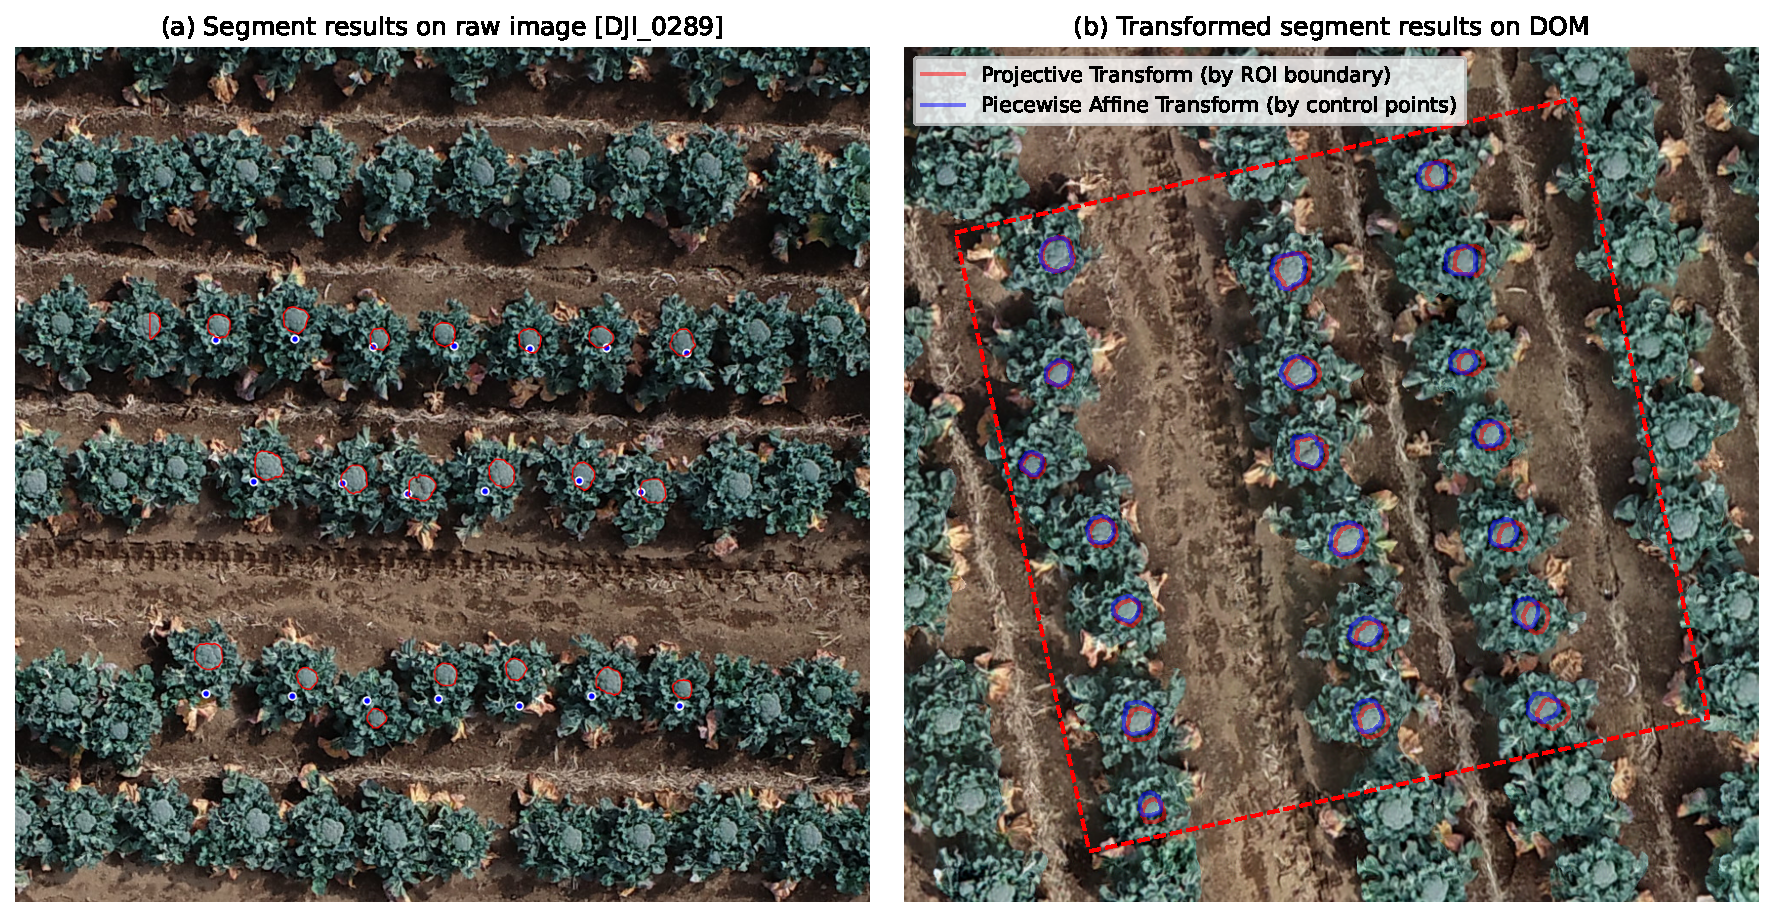
\includegraphics{figures/xrs/trans_compare_220331_114_DJI_0289.pdf}
    }
  \end{center}
  \caption[Head segmentation forward location comparison between projective and piecewise affine transformation]{
    Head segmentation forward location comparison between projective (in Chapter 3) and piecewise affine transformation (this chapter). (a) is the head segmentation results on the raw image. They are forward transformed to corresponding positions on the \gls{dom} using two different transformations.
  }
  \label{fig:xrs3}
\end{figure}

\begin{figure}[htb!]
  \begin{center}
    \resizebox{\textwidth}{!}{
      \includegraphics{figures/xrs/validation4automl.pdf}
    }
  \end{center}
  \caption[Validation for the AutoML calibration model]{
    Validation for the AutoML calibration model.
  }
  \label{fig:xrs4}
\end{figure}

\begin{figure}[htb!]
  \begin{center}
    \resizebox{\textwidth}{!}{
      \includegraphics{figures/xrs/aerial_matched_compare_220405_29.pdf}
    }
  \end{center}
  \caption[The closest matched broccoli head template 3D model]{
    The closest matched broccoli head template 3D model to each aerial segmentation results. Different colors represent different broccoli heads.
  }
  \label{fig:xrs5}
\end{figure}


\section{Discussion}

\section{Conclusion}